\section{\label{sec:back:cml}\glsfmtlong{cml-glossary}}

While parallelism is often the best (perhaps only) way to achieve improvements in execution time for different algorithms once an efficient sequential implementation has been created, it is a notoriously challenging affair \cite{Shun2017}.  When working at the level of directly manipulating threads, such as using the \texttt{pthreads} found in POSIX-compliant operating systems \cite{posix2017}, programmers are exposed to a high level of risk of inadvertently introducing concurrency bugs, such as data races, deadlocks and livelocks.  A panoply of approaches to overcoming this challenge, both theoretical and practical, have been proposed and developed over the years, with varying degrees of success, \eg{} \cite{Boyapati2002,Bocq2012,Seinstra2004}.  Many, perhaps most, large-scale programming languages that use a runtime include some form of parallelism simplification within their standard libraries, \eg{} the Executor system in Java \cite[Ch. 4]{Fernandez2012}, and Swift \& Objective-C's Grand Central Dispatch \cite{Maskrey2018}.

Most simplifications fairly directly target either data-parallelism by simultaneously applying the same operation over multiple elements in arrays, \eg{} SIMD instructions in CPUs \cite{Hughes2015}, or task-parallelism following the fork-join model \cite{McCool2012}.  These simplifications can be very useful, but not all instances of potential parallelism fit neatly into their models.  For example, algorithms that are well-modelled by the \gls{csp} and \gls{actor} models, such as those explicitly centred around concepts of message passing, are not necessarily easy to express using either SIMD or fork-join instructions.

\Gls{cml} \cite{Reppy1991,Panangaden1997} is an approach to concurrent programming originally developed by John Reppy (based on his earlier \emph{Pegasus Meta-Language} \cite{Reppy1988}).  \Gls{cml} was created to provide a framework for writing concurrent programs with synchronous communications on uniprocessor machines,\footnote{In fact, under-the-covers the original implementation \emph{relied} on the fact that the processor was single-core.} and was later extended to permit parallelism \cite{Reppy2009a}.  It was developed originally for Standard ML of New Jersey\footnote{\url{https://www.smlnj.org/}} (where ML refers to the earlier programming language \emph{Meta Language}), whence the ML part of the name, but its concepts have subsequently appeared elsewhere.  The basic concept of communicating via channels has experienced a renaissance lately, likely due at least in part to its inclusion as a core feature of Go \cite{Meyerson2014}, but \gls{cml} has a more advanced system that Go (at the time of writing) does not fully support.

\begin{figure}
    \centering
    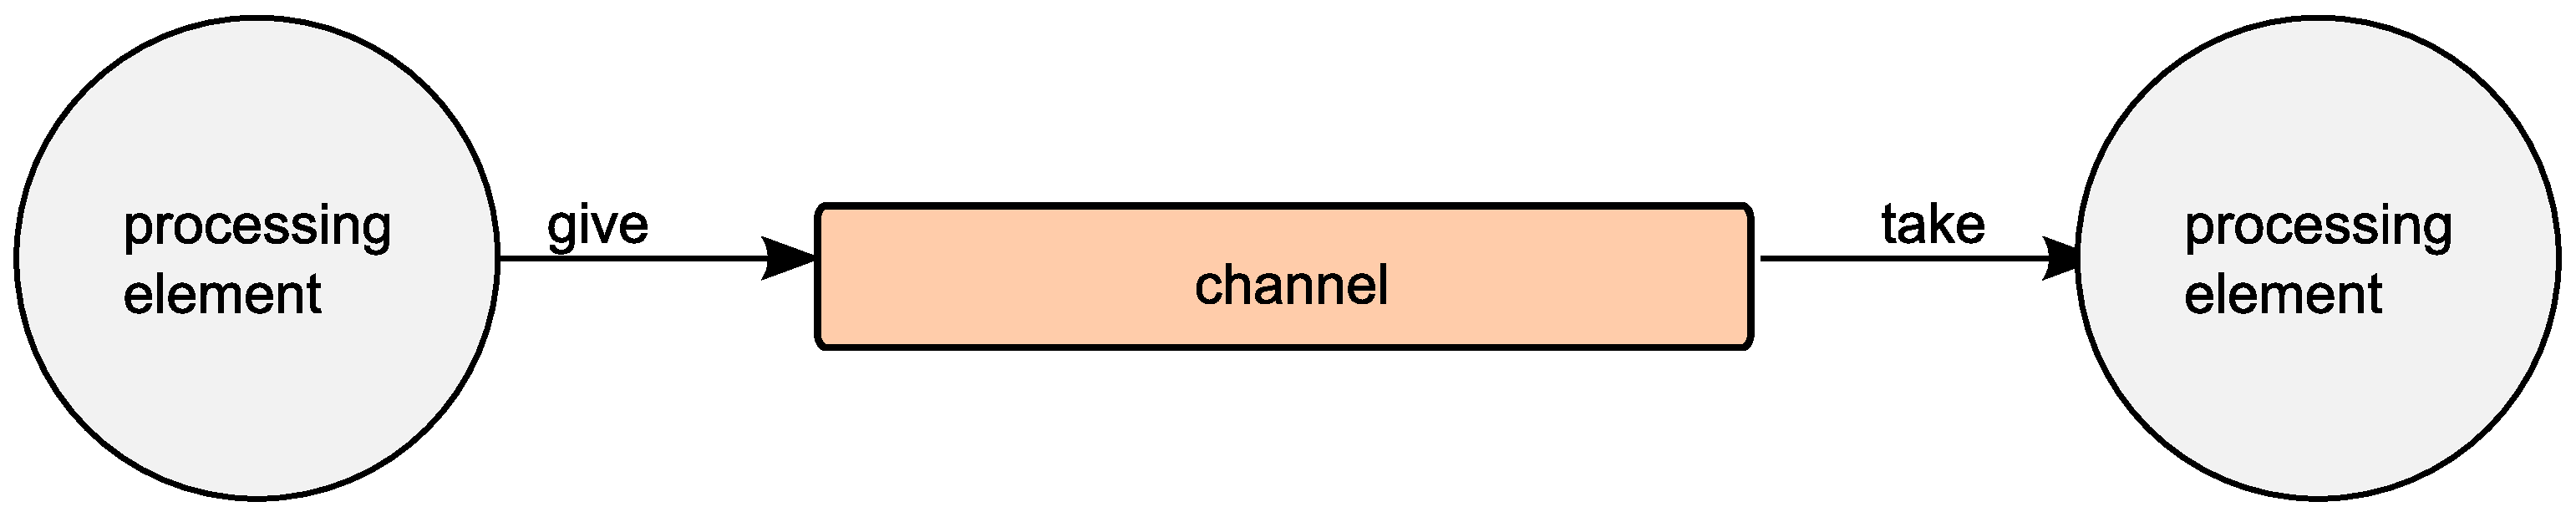
\includegraphics[width=\textwidth]{chapters/background/images/cml_exchange.eps}
    \caption[Diagram of the message-passing primitive in \glsentrylong{cml-glossary}]{In \gls{cml}, logical processing elements synchronously exchange values over channels.  When one processing element offers to give a value on a channel, and another offers to take a value on the same channel, they `rendezvous' and exchange the value as a passed message.}
    \label{fig:back:cml_exchange}
\end{figure}

\Gls{cml} is designed to avoid many of the difficulties with concurrency that arise in traditional sequential-first programming, where the use of locks, mutexes and semaphores \etc{} are frequently required, and often lead to the introduction of problems such as live-/deadlocks, data races and extreme resource contention.  This is achieved by changing the approach to concurrent programming to one of logically separate, internally sequential processing elements that share data as required by ``passing messages''\footnote{This is the logical concept, but there is not strictly any specific required software implementation.} between themselves, following similar fundamental principles to \glspl{actor} and \gls{csp}.  In \gls{cml}, these logical processing elements are referred to as \emph{threads} (a somewhat distinct concept from the threads found in many popular programming languages), and they exchange messages over channels \emph{synchronously} (called \emph{rendezvous}), \ie{} there is a temporal overlap for the same channel between one thread offering to send, and another to receive.  The first to offer blocks until the second makes its offer.  When two processes are offering appropriately on either side of an exchange, rendezvous takes place and the proffered datum (conceptually) ``moves'' from the sender to the recipient.  \Cref{fig:back:cml_exchange} provides a visualisation of this concept.

Reppy describes a concurrent program as one that supports multiple sequential sub-programs conceptually executing separately in parallel but interacting through shared resources to achieve a common goal.  \Gls{cml} is concerned with the scenario where said interactions are explicit, and to facilitate that \enquote{\gls{cml} takes the unique approach of supporting \emph{higher-order concurrent programming}} (emphasis Reppy's), whereby communication and synchronisation are made into first-class members of the language, similar to how functional programming languages made functions into first-class members of themselves \cite[Preface]{Reppy2007}.